\documentclass{article}

% Preâmbulo mínimo
\usepackage[brazilian]{babel}
\usepackage{graphicx}
\usepackage{booktabs}
\usepackage{amsmath}
\usepackage{natbib}

\title{Relatório Analítico: Distribuição da Temperatura Diária em Nova York}
\author{Yannis Boz Papazoglou}
\date{\today}

\begin{document}

\maketitle

\section{Origem e Descrição dos Dados}

Os dados analisados neste trabalho foram obtidos a partir do conjunto de dados nativo do R denominado \texttt{airquality}, que registra medições diárias da qualidade do ar em Nova York entre maio e setembro de 1973. O conjunto contém um total de 153 observações relativas a 6 variáveis.

Neste relatório, o foco da análise é a variável temperatura (\texttt{Temp}), aferida em graus Fahrenheit (°F). Após a inspeção dos dados, verificou-se que não há valores ausentes (\textit{missing values} ou \texttt{NA}) para a variável temperatura ao longo de todas as 153 medições realizadas no período. As análises e visualizações foram geradas utilizando o ambiente estatístico R \citep{Rstat}.

\section{Análise Estatística e Visualização}

Os dados de temperatura foram agrupados por mês para o cálculo das médias mensais. A Tabela~\ref{tab:resumo} apresenta o número de dias medidos e a temperatura média correspondente para cada um dos cinco meses analisados.

\begin{table}[htbp]
  \centering
  \caption{Média mensal da temperatura e número de medições (maio a setembro de 1973).}
  \label{tab:resumo}
  \begin{tabular}{lrrc}
    \toprule
    Mês & Mês (Extenso) & Dias Medidos & Média (°F) \\
    \midrule
    5 & Maio & 31 & 65,55 \\
    6 & Junho & 30 & 79,10 \\
    7 & Julho & 31 & 83,90 \\
    8 & Agosto & 31 & 83,97 \\
    9 & Setembro & 30 & 76,90 \\
    \bottomrule
  \end{tabular}
\end{table}

A média amostral $\bar{X}_m$ para cada mês $m$ é calculada de acordo com a Equação~\eqref{eq:media}:

\begin{equation}
  \bar{X}_m = \frac{\sum_{i \in D_m} X_i}{N_m}
  \label{eq:media}
\end{equation}

Na Equação~\eqref{eq:media}, o denominador $N_m$ conta estritamente o número de observações válidas (não ausentes) registradas no mês $m$, garantindo que eventuais valores faltantes no conjunto de dados não distorçam a média aritmética calculada pelo script \texttt{resumo.sh}.

A distribuição espaço-temporal da temperatura ao longo dos meses pode ser observada na Figura~\ref{fig:boxplots}, que exibe os diagramas de caixa gerados para o período. A geração de gráficos estatísticos e manipulação dos dados baseou-se em literaturas consolidadas de R \citep{wickham2016r}.

\begin{figure}[htbp]
  \centering
  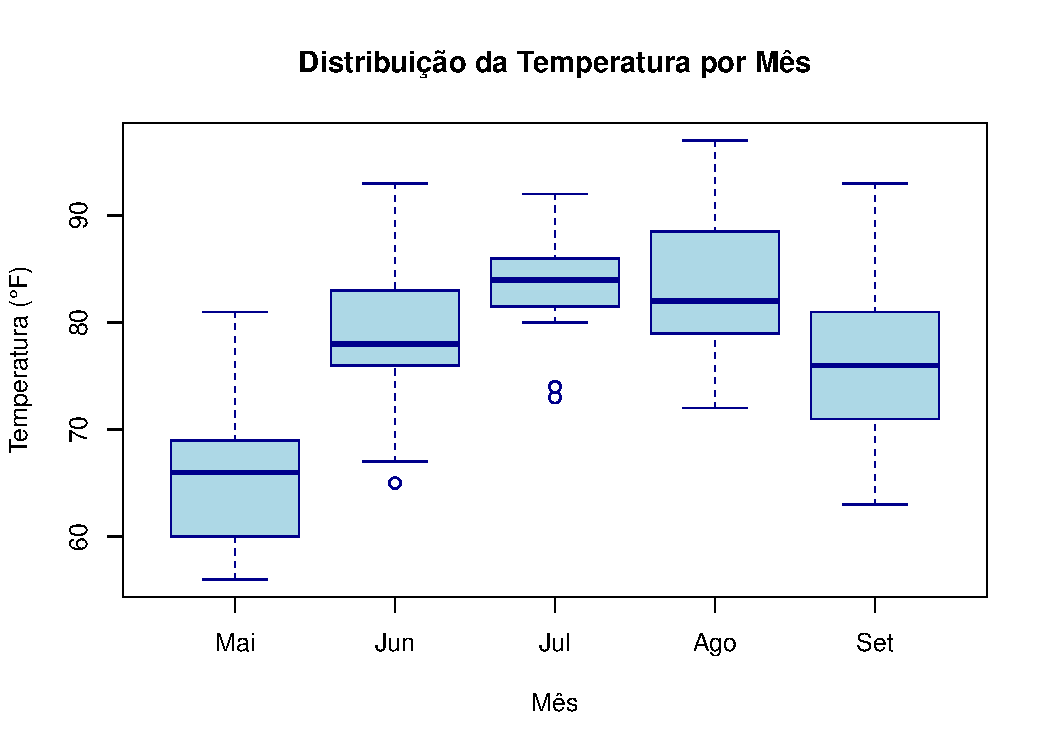
\includegraphics[width=0.8\textwidth]{figura.pdf}
  \caption{Distribuição da temperatura mensal (°F) de maio a setembro de 1973.}
  \label{fig:boxplots}
\end{figure}

\section*{Declaração de Uso de IA}

Durante a elaboração deste trabalho, a ferramenta de inteligência artificial generativa ChatGPT/Gemini foi utilizada para auxílio na estruturação sintática do documento em \LaTeX, depuração de comandos de pacotes (\texttt{booktabs} e \texttt{natbib}) e ajustes nos blocos do arquivo de referências BibTeX. Todas as contagens, médias e a geração do arquivo PDF foram executadas via scripts próprios no ambiente Linux/WSL e conferidas manualmente no terminal.

\bibliographystyle{plainnat}
\bibliography{referencias}

\end{document}
